\section{Redes de eSalud}

Se define como un conjunto de nodos especializados con capacidad operativa para brindar servicios de eSalud, garantizando atributos de calidad, estandarización, interoperabilidad, privacidad y seguridad \cite{wilson2017}. La arquitectura base de cada nodo de la red es de tipo agregado con \textit{micronodos} agrupados funcionalmente para brindar un conjunto de servicios que pueden ser consumidos por otros nodos,creando así estructuras funcionalmente complejas. Los nodos de más alto nivel de abstracción son lo que tienen capacidad de ofrecer servicios de eSalud.

\begin{figure}
 \centering
 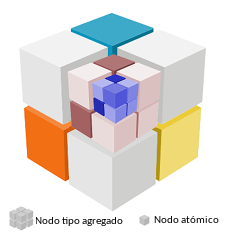
\includegraphics[width=80mm, height=83mm]{concepto_red_esalud.png}
 \caption{Vista conceptual de la arquitectura de una red de eSalud en OpenSITEM}
 \label{elementosred}
\end{figure}

De acuerdo a las recomendaciones del grupo GITEM, la descripción de la arquitectura de cada nodo - así como la de la red, puede obtenerse de manera emergente a partir de métodos definidos como el Architecture Development Method (ADM) de The Open Group o similares. Se aclara que OpenSITEM no es una plataforma para prestación de servicios de eSalud sino para la descripción de nodos de la red - a cualquier nivel de abstracción, a partir del modelo de agregación. 

\subsection{Caracterización de Nodos para Redes de eSalud}

Diferentes organizaciones \cite{ops2011},\cite{oms2016}, \cite{ituoms2012}, han determinado que los proyectos de eSalud incluyen nodos de naturaleza diversa; por ejemplo, médica, tecnológica, de recurso humano, financiero, estratégico, de organización, de política y de infraestructura. Debido a esta pluralidad el equipo de diseño y planeación de redes de eSalud del grupo de investigación GITEM, se encontró con el obstáculo de no disponer de información de calidad de los nodos potenciales que harían parte de la red. Para poder sortear dicho obstáculo fue necesario proponer un \textit{reducido} de nodos\footnote{El reducido es un conjunto finito de nodos con capacidad de entregar una funcionalidad contractualmente definida relacionada con la eSalud} y una descripción de la arquitectura de cada uno de ellos, de tal manera que se pudiese recopilar datos basados en modelos de información.

Los primeros resultados del estudio de campo mostraron que un servicio - con posibilidad de ser implementado en un modelo de eSalud, requiere de la integración jerárquica de nodos. En OpenSITEM existen dos tipos de nodos: (1) atómicos: aquellos que ofrecen un servicio cohesivo que no abarca un caso de uso de dominio  y (2) agregados: que articulan nodos (atómicos o agregados) para brindar capacidad funcional a nivel de caso de uso de negocio. Si se considera que el modelo de dominio gira en torno a los servicios de eSalud, el nodo agregado que lo provee se denominará \textit{macronodo}.

Un nodo atómico está caracterizado por atributos (propiedades) e interfaces, estás últimas definidas como los puntos de acceso en donde los servicios del nodo son expuestos para ser consumidos\cite{theopengroup2016}. Un nodo agregado está definido por la 










En este sentido, el grupo de investigación decide desarrollar un proyecto enfocado en la caracterización multidominio de los sistemas de salud para poder determinar la capacidad que estos presentan para poder desarrollar eSalud. 

La fase actual del SITEM se centra en varios componentes: médicos, tecnológicos, administrativos, humanos y financieros. Sin embargo, debido al perfil de profesionales que han participado en el desarrollo, los elementos tecnológicos han sido mejor caracterizados hasta el momento.

\begin{figure}
 \centering
 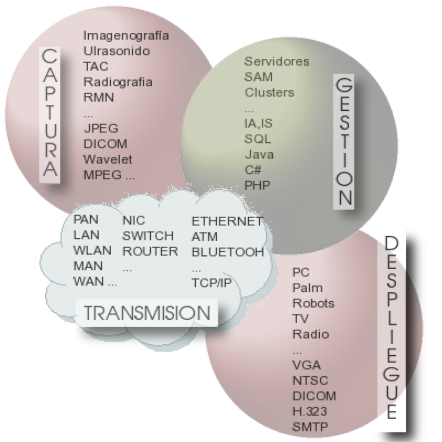
\includegraphics{red_1.png}
 \caption{Componentes en un Sistema de eSalud. Fuente: OMS/ITU}
 \label{subcomponentes}
\end{figure}

Para facilitar el análisis y modelado en la dimensión tecnológica, un sistema de eSalud - con enfoque de Telemedicina, puede reducirse a cuatro subsistemas: \cite{aparicio2003}

\begin{itemize}
 \item \textbf{Subsistema de Captura de datos:} Conformado por los dispositivos de hardware, los protocolos y aplicaciones software que trabajan conjuntamente para transformar información médica en datos susceptibles de ser administrados usando técnicas digitales.
 \item \textbf{Subsistema de Transmisión de Datos:} Hacen parte de este subsistema los dispositivos de hardware, las tecnologías de interconexión, los protocolos y aplicaciones que permiten estructurar redes de transmisión de datos digitales de una manera fiable en tiempos aceptables para un servicio específico.
 \item \textbf{Subsistema de Gestión de Información:} Dispositivos de hardware - computadores, sistemas de almacenamiento masivo, etc; y  sistemas de información que almacenan, procesan, distribuyen, analizan, integran y producen información con base en los datos de los subsistemas de captura, históricos y de pronóstico.
 \item \textbf{Subsistema de Despliegue de información:} Elementos de hardware (pantallas, transductores, sistemas de audio, etc), aplicaciones software y protocolos asociados que permiten recibir y reproducir información médica. 
\end{itemize}

Todos ellos necesariamente interrelacionados por medio de interfaces y protocolos definidos. El uso de estándares abiertos es de vital importancia para permitir que estos subsistemas puedan ser interoperables. Esto se ha logrado en gran medida en el subsistema de transmisión de datos pero aún se encuentran serios problemas en los demás, debido al sinnúmero de patentes - y protocolos propietarios, que las empresas fabricantes de dispositivos médicos aún ostentan.